Recall the paint factory problem 
%
\begin{flalign}
	\maxi z = \ & 5x_1 + 4x_2 \label{p1c1:eq:constM1}\\
	\st & 6x_1 + 4x_2 \leq 24 \label{p1c1:eq:constM2}\\
	& x_1 + 2x_2 \leq 6 \\
	& x_2 - x_1 \leq  1 \\
	& x_2 \leq 2 \\
	& x_1, x_2 \geq 0,
\end{flalign}
%
where $x_1$ representes the amount (in tons) of exterior paint produced, and $x_2$ the amount of interior paint produced. This is a simple linear problem that has been used as an illustrative example throughout the lecture notes. 

To demonstrate some typical structures in integer programming models, we now add two modifications to the problem, namely
%
\begin{itemize}
    \item Piecewise linear functions: the profit for exterior paint depends on the amount produced. The profit for the first ton produced is 7 (\$1000/ton), while the next ton can only be sold at a profit of 5, the third for a profit of 3 and the fourth ton only makes a profit of 1. 
    \item Logical constraints: the factory has to produce at least 1.5 tons of at least one of the two paint types, that is, either $x_1 \ge 1.5$ or $x_2 \ge 1.5$ must hold.
\end{itemize}

As seen in Fig. \ref{p1c8:fig:E86-plot}, these modifications result in a nonlinear objective function and a nonconvex feasible region. Using additional integer/binary variables, formulate and solve the problem as a mixed-integer linear problem.

\begin{figure}[h]
	\centering
	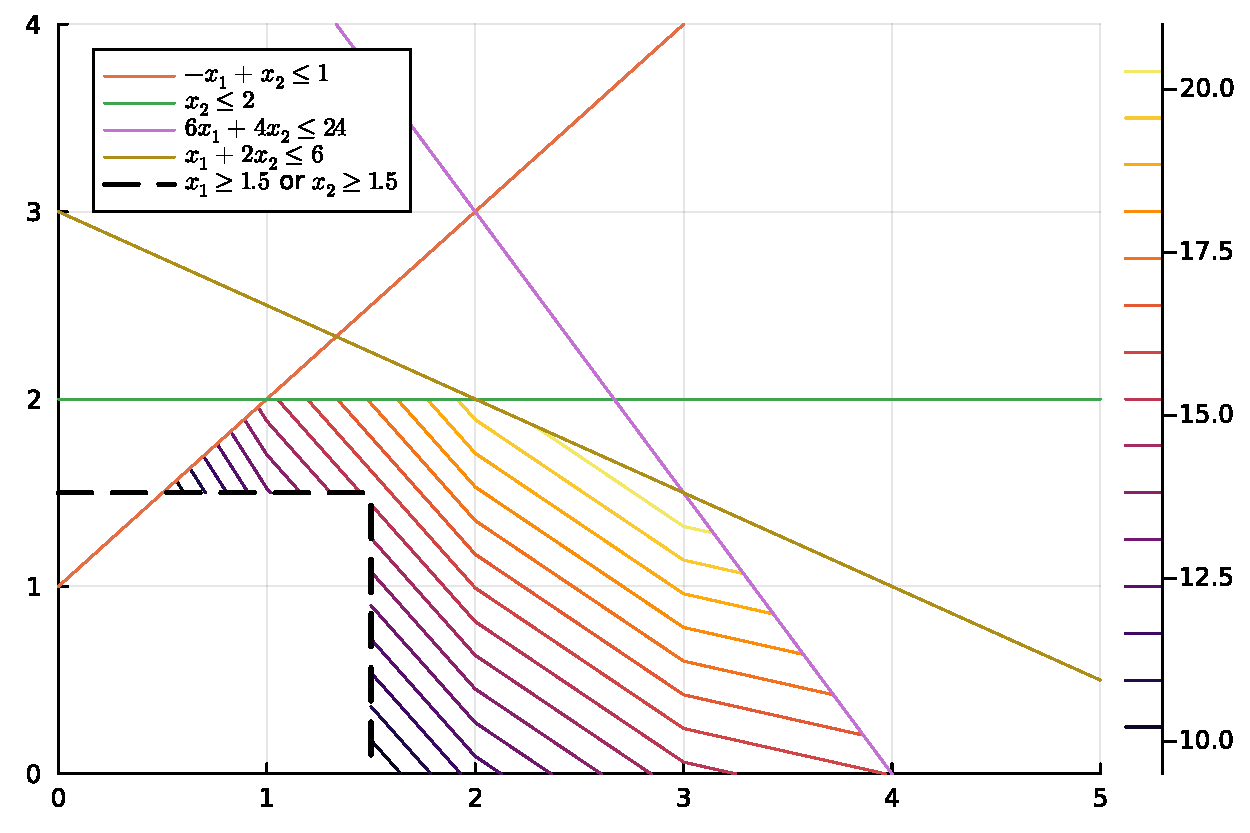
\includegraphics[width=0.5\textwidth]{part_1/chapter_8/figures/E86-plot.pdf}
	\caption{The feasible region of the problem, and the contours of the objective function} 
    \label{p1c8:fig:E86-plot}
\end{figure}